%!TEX root = ./Intro_to_CC.tex

\section{Problem 3: Hydronium cation}
\label{sec:problemIII}
\subsection*{Planar hydronium cation}

This exercise covers how to perform geometry optimizations.
Specifically, we will relax the \ch{H3O^+} molecule starting from an initial planar guess for the geometry. 

\begin{enumerate}

  \item The planar \ch{H3O+} geometry has been provided in the file \Verb{geom_planar.xyz}.
  \begin{gaussinput}[title=Contents of \Verb{geom_planar.xyz}]
O    0.00    0.00   0.00
H    0.92   -0.53   0.00
H   -0.92   -0.53   0.00
H    0.00    1.06   0.00

  \end{gaussinput}
  
  \item We'll create a Psi4 molecule based on the example provided in Problem~1.  
  Use the \Verb{HF} level of theory and the \Verb{6-31G(d,p)} basis set. 
  We also need to set the values for charge and multiplicity. 
  Because \ch{H3O+} carries a charge, we want to tell Psi4 explicitly what values to use for these fields. 
  \begin{description}[font=\ttfamily\upshape]
    \item[charge] The program will guess the charge of the molecule, but this value can be explicitly set. 
    \item[multiplicity] As above, the program will try to guess the spin multiplicity of the system (\( 2\mtext{S}+1 \), where \( \mtext{S} \) is total spin). This should always be an integer. It can be explicitly set when necessary. 
  \end{description}
  We want to relax the geometry and perform the vibrational analysis of the ion. 
  Rather than calculating energy with \pyinline{psi4.energy()}, we'll let Psi4 optimize the geometry, then ask it to perform a frequency analysis on the optimized molecule. 
  This is done by calling \pyinline{psi4.optimize()} followed by \pyinline{psi4.frequency()}, specifying the appropriate method. 
  This is set up for you in the second code cell in the section for Problem~III. 
    
  \item Once the calculation is complete, we will visualize the results in JupyterLab. 
  Execute the first few cells of the section until you get an output that shows you the molecule. 
  This cell also outputs the total energy of the ion. 
  Note the command that outputs this value. 
  Also note that the molecule doesn't show bonds between any of the atoms. 
  What does the fully relaxed structure look like? 
  You can use your mouse to click and drag on the molecule to rotate it. 
  Do you believe that this is the structure of \ch{H3O+} in the gas phase? 
  % Save a picture of the ion.
  
  \item We'll use two additional cells to define bonds between the oxygen and all three hydrogens and to reformat the vibrational information so we can visualize it. 
  The final cells in this section of the notebook will show the corrected structure and list the normal modes/vibrations with their IR intensity, sorted by wavenumber (\unit{\wn}). 
  Click through the spectrum to animate some of the vibrations. 
  You can select all of the vibrations by clicking the menu icon \( (\vdots) \) in the upper right corner of the output view window and using the dropdown menu for ``Normal Mode''. 
  You should see that one of the frequencies is negative -- select the normal mode to which it corresponds. 
  In the discussion section (at the end of the notebook), include this table and indicate what kind of molecular motion each vibration corresponds to. 

\end{enumerate}


\subsection*{Pyramidal hydronium cation}

Next, repeat the calculations for a pyramidal hydronium cation: 
\begin{gaussinput}[title=Contents of \Verb{geom_pyramidal.xyz}]
O    0.00   0.00   0.00 
H    0.92  -0.53  -0.66 
H   -0.92  -0.53  -0.66 
H    0.00   1.06  -0.66 

\end{gaussinput}
It's probably easiest to copy the group of cells from the planar section, then work through each one and modify the ``planar'' values to be ``pyramidal''. 
Visualize the results again using the steps from the previous section. 
You should see the \ch{H3O+} in a pyramidal conformation now.  
Note again the total energy of the ion and compare it with the planar structure in your discussion. 
Which conformation has lower energy? 
Next, view the vibrations table and spectrum. 
If calculations were done properly, all vibrations should have positive wavenumbers. 
Describe again in the discussion section the motion the vibrations correspond to. 

\subsection*{Potential-Energy Surface Scan}

In the final problem, we are going to inspect the potential-energy surface of the hydronium ion along its umbrella mode. In the planar cation problem, you have seen that the negative\sidenote{In fact, it is imaginary, \(i\) is dropped by convention} frequency corresponds to such an ``umbrella'' mode. 

Again, many of the steps have been set up for you already. 
In the main folder, you should see a file called \Verb{h3o.zmat}.
If you open it, you should see that the \( xyz \)-cartesian coordinates have been replaced with a \( z \)-matrix. 
The \( z \)-matrix allows precise control of the geometry within single calculations.

\makeatletter
\begin{gaussinput}[title=\(z\)-matrix in the PES input file]
@H                         
O   1 a                    
H   2 a   1 HOX            
H   2 a   1 HOX   3  120.0 
H   2 a   1 HOX   3 -120.0 

\end{gaussinput}
\makeatother
  
\begin{marginfigure}[-12\baselineskip]
  \centering
  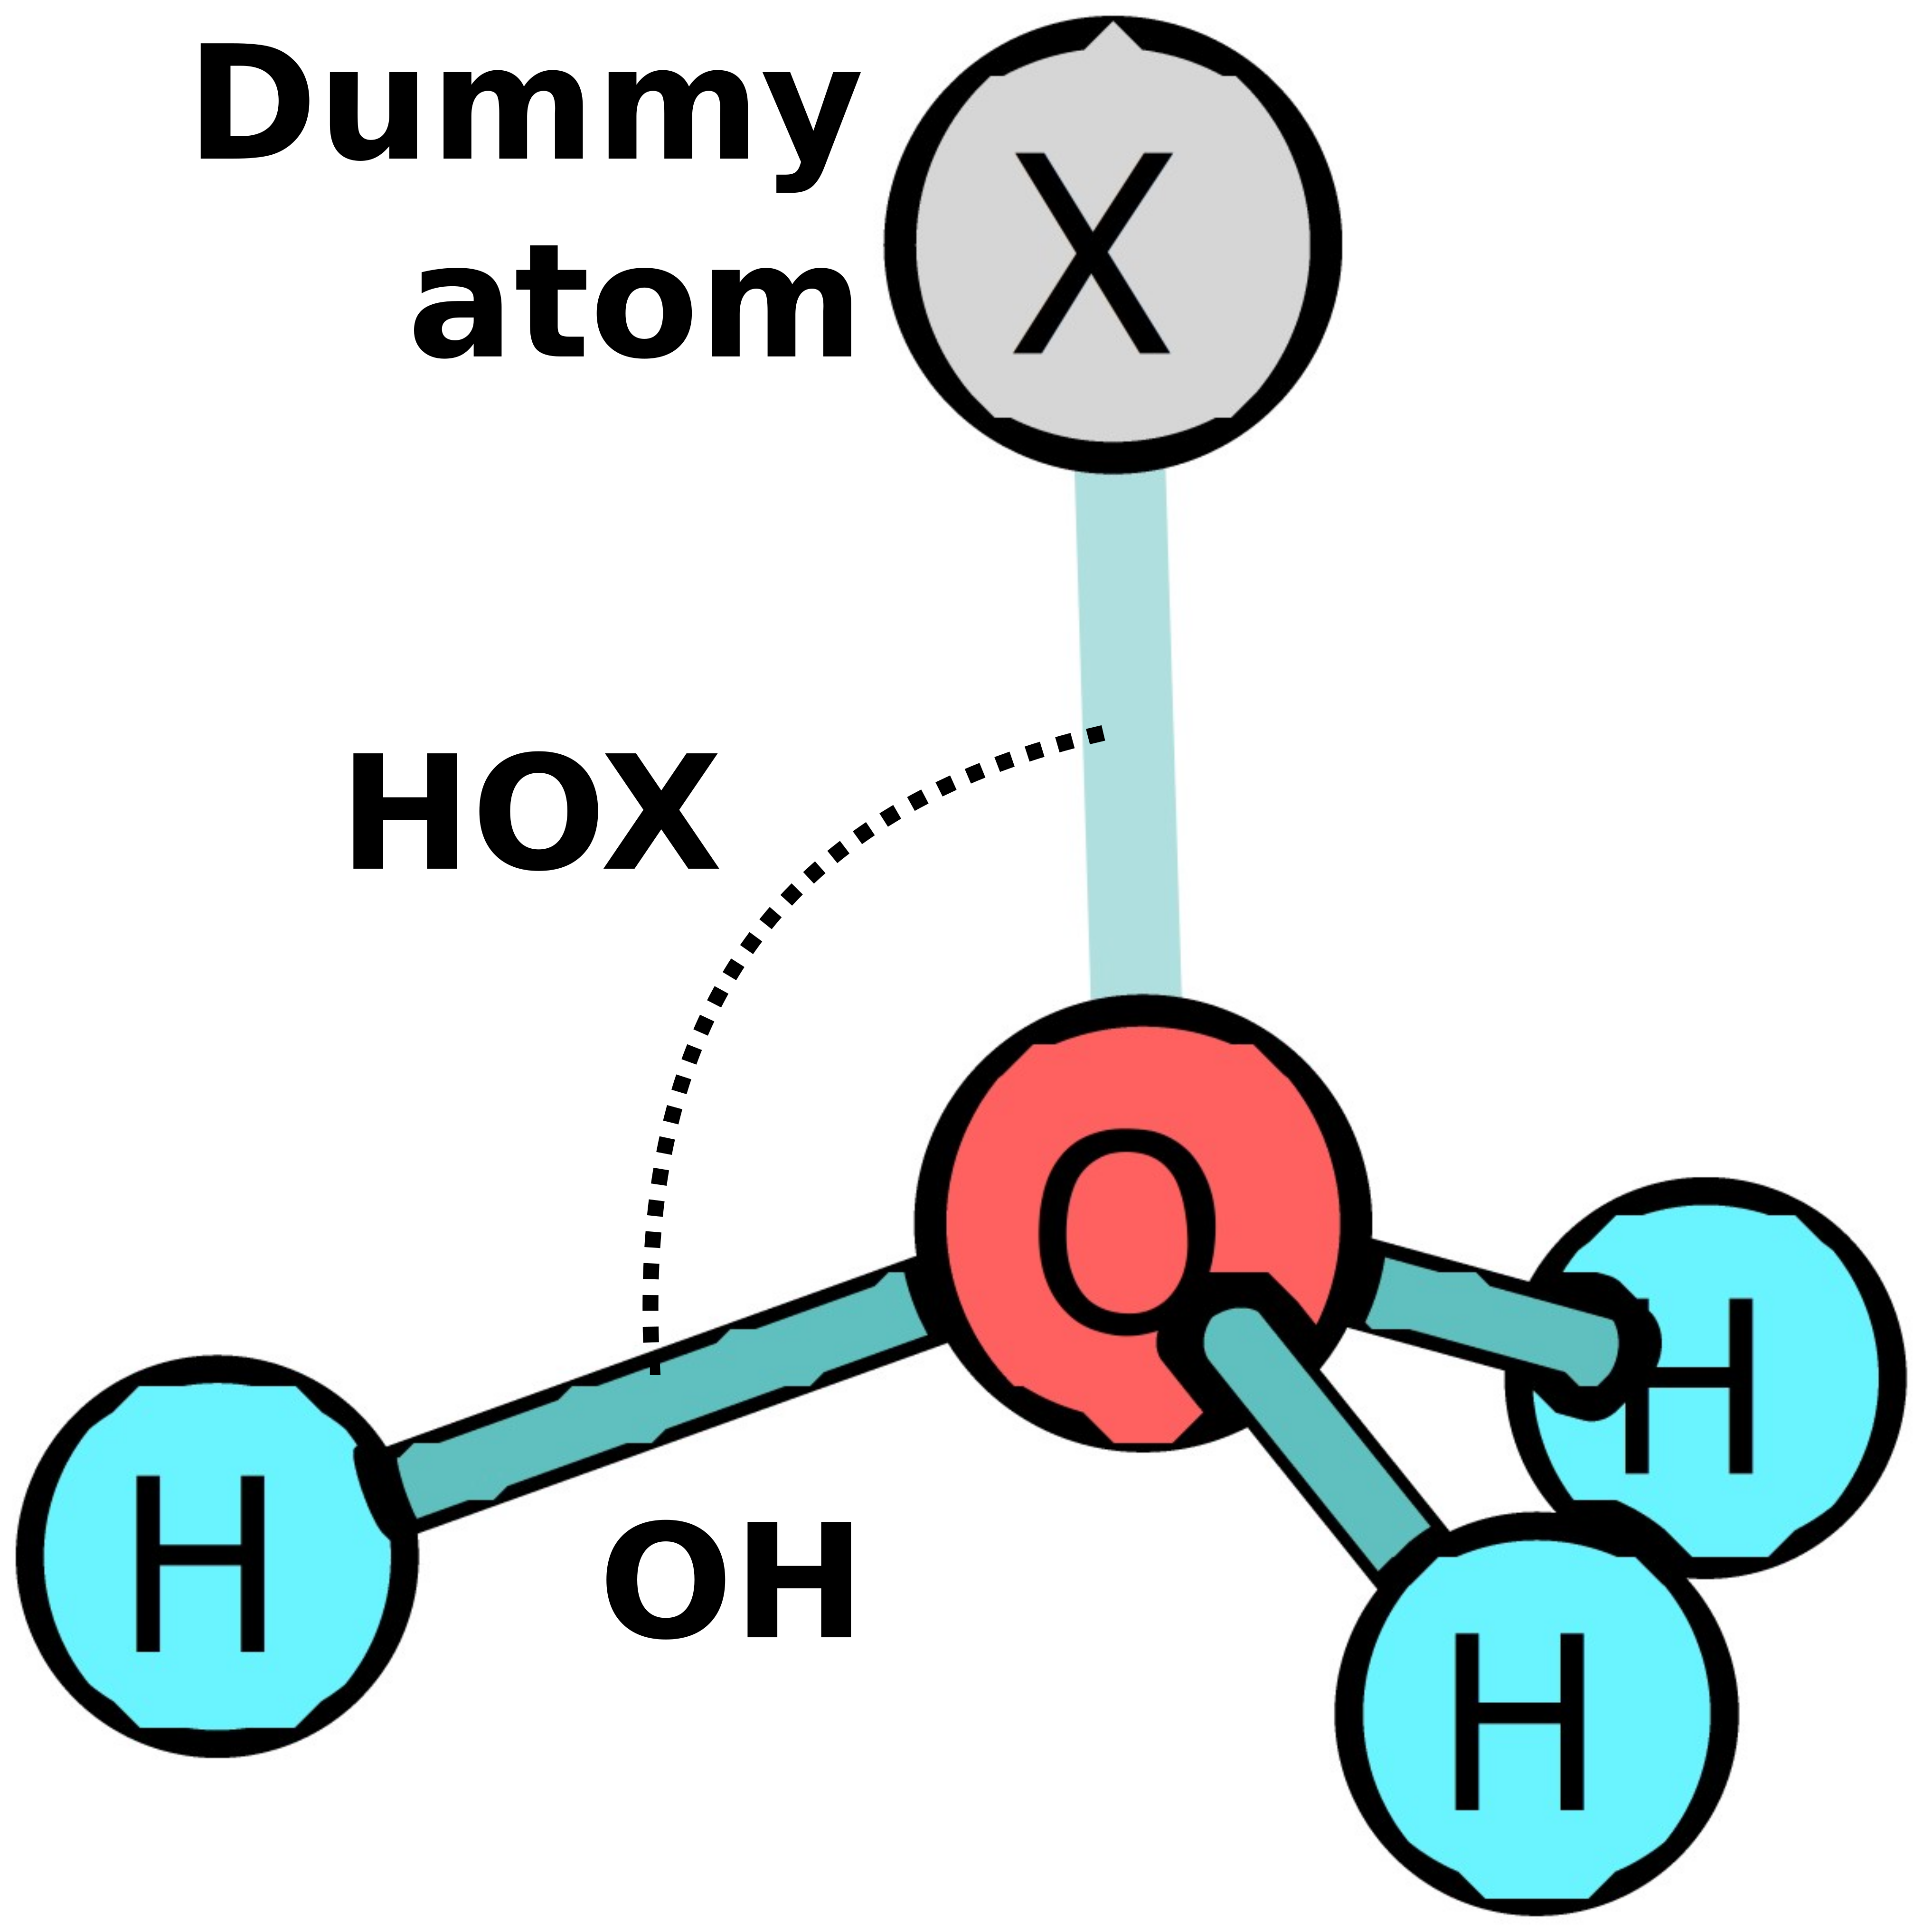
\includegraphics[width=0.75\textwidth]{pics/zmat.png}
  \caption{Definition of hydronium ion internal coordinates. 
    The calculations perform a scan along the \ch{X-O-H} coordinates for all three hydrogens from \SIrange{135}{90}{\degree}. 
    The \ang{120} dihedral angle indicates the relative position of hydrogen atoms.}
  \label{fig:internal_coords}
\end{marginfigure}
The first column shows the atom identity, the second specifies to which atom it's bonded, the third column is the bond length, the fourth and fifth give a second reference atom and the angle between the line atom and the two reference atoms, final two columns specifies the dihedral angle between the prior bond and a third reference bond. 
\makeatletter @H \makeatother is a dummy (non-existent) atom that enables control of the umbrella motion. 
\Cref{fig:internal_coords} explains the \( z \)-matrix graphically. 


\begin{enumerate}
  \item First, calculate the \ch{O-H} distance using the functions defined in the first cell of this section and the optimized pyramidal geometry from the previous section. 
  Set the value of \Verb{a}\sidenote{Defined in the input file} in the input molecule to this value. 
  \item Next, run a set of energy scans using Psi4. 
  You should write a loop to perform an energy calculation for different values of the \ch{X-O-H} angle, saving the energy every \ang{1} from \SIrange{90}{135}{\degree}.\sidenote{
    Remember, Psi4 reports energy in atomic units, so you'll need to think about how to compare data between the PES scan and the data imported by cclib.} 
  \item When the calculations are finished, plot the resulting potential-energy surface. 
  Discuss these results in your report.  
  The PES for angles below \ang{90} is the mirror image of the values above \ang{90}. 
  Use \unit{\kcal\per\mol} instead of \unit{\hartree} in the report. 
  \item Localize the lowest-energy and transition structure along the PES and calculate the reaction barrier of the internal flip of the hydronium ion. 
  Whereas the energy of the pyramidal ion is comparable with the minimum on the PES, the energy of the optimized planar cation and the local maximum on the PES is different. 
  Why? Compare the geometries. 

  \item In the final step, rerun the calculations using the MP2 method and compare your results. 
  You'll need to rerun the geometry optimization (for the pyramidal molecule) using the MP2 level of theory so you get the right bond length to run the PES scan of the umbrella mode. 
  You do not need to save the output file; it is possible to get geometry data directly out of the Psi4 output. 
  This is left as an exercise for the student. 
  Try plotting both PES scan curves in one plot to compare methods. 
  Look at the difference in final energies and the difference in the barrier energy for the two methods. 
\end{enumerate}

\section*{Lab report}

For the lab report, please prepare following data.\sidenote{This is the bare minimum requirement; there are couple of open questions in the text that you should try to assess.}
All of this can be done in the Discussion section of the Jupyter notebook. 
When you are finished, save a copy of your report to the folder \Verb{shared/submissions}. 

\begin{enumerate}
  \item Plot the Total Energy vs. number of basis functions for a hydrogen atom for all methods used in Problem 1. 

  \item Plot the binding curves for HF using Hartree-Fock and PBE1PBE methods. Find the minimum distance and compute the atomization energy. 
  Plot the dipole moment as a function of the bond distance. 
  Remember, multiple sets of \emph{x-y} data can be plotted with \Verb{plt.plot(x1, y1, x2, y2)}, where \Verb{x1}, ... are the various lists of \emph{x} and \emph{y} data. 

  \item Prepare tables listing molecular vibrations in a hydronium ion in planar and pyramidal geometries. 
  Make sure the wavenumbers are shown for all molecular vibrations. 

  \item Plot the PES along the HOX coordinate using HF and MP2 methods. 
  Use \unit{\kcal\per\mol} for the \( y \)-axis. 
  Compute the heigh of the barrier separating two pyramidal structures (the energy required to pass over the planar intermediate on the PES). 
\end{enumerate}


